\chapter{时间序列预测建模框架
% \footnote[11]{
%     本章成果已开源在:https://github.com/Analytics-for-Forecasting/OpenForecasting.
% }
\label{sec:chapter.univ}
}
\section{引言}
时间序列预测建模技术是能源、交通、金融和工业生产等众多重要现实管理应用领域的重要支撑技术。
在不同场景中,时间序列数据表现出动态机制不确定、模态表现不相同、数据规模不一致的高度复杂特征。
因此,时间序列预测问题是一项颇具挑战和相当复杂的问题。
如何针对不同场景构造准确、稳定和鲁棒的时间预测模型是众多研究者与工作者所关注的重要课题。

针对时间序列预测建模问题,各种预测建模技术推陈出新。其中,以深度神经网络为代表的深度学习预测建模技术因其优异的预测性能成为了近年的研究热点,涌现出大量基于深度神经网络模型的技术应用研究\cite{wuImproved2019,zhaoDeep2017,sezerFinancial2020,caiDayahead2019,lindbergLongterm2019,shiDeep2018,laptevTimeseries2017,wangTraffic2016,xiaoShortterm2019}。
但在复杂多变的不同应用场景中,这些深度学习预测建模方法往往无法给予稳定的性能保证和一致的性能优势。
原因在于,作为一种基于复杂神经网络结构构造的学习预测模型,深度学习预测模型往往具有远超传统机器学习方法或统计方法的参数设置,同时,传统深度学习预测模型的梯度下降迭代训练权重参数方法进一步降低了模型构造的效率,
使得深度学习预测模型的构造过程面临建模效率低、模型选择难的问题。

作为深度学习预测建模技术应用与发展的关键,深度学习预测模型的高效构造与选择问题受到学术界与工业的广泛关注。为便捷构造深度神经网络模型,Google、Meta(Facebook)和Microsoft分别推出了TensorFlow\cite{abadiTensorflow2016}、Pytorch\cite{paszkePytorch2019}和CNTK\cite{seideCNTK2016}等神经网络模型构造框架,通过封装常用深度神经网络基础结构(如卷积核结构、循环层结构和线性结构),集成多种先进梯度下降训练算法和矩阵运算与处理算法,为深度学习模型的深入研究与广泛应用提供了框架。
为解决深度学习模型复杂的超参数搜索与优化问题,Bennet等\cite{bennetNevergrad2021}提出了一种开放优化框架Nevergrad,通过内置贝叶斯优化、粒子群优化和差分进化等优化算法为深度学习模型参数搜索与优化提供了便利平台。
Akiba等\cite{akibaOptuna2019}基于贝叶斯类优化方法提供了一套运行定义(Define-by-run)模型的优化框架OPTUNA,通过更个性化的搜索空间定义接口,支持搜索范围可根据采样结果自适应变动的复杂搜索设置。
Liaw等\cite{liawTune2018}通过集成Nevergrad和OPTUNA等优化框架,提供了一套内置多种优化算法的分布式优化平台Ray,进一步提高了模型参数优化的效率。

然而,这些建模与优化框架技术主要关注于广义建模技术中的特定环节,欠缺针对时间序列预测领域的建模考量。
在面对复杂多变的时间序列管理应用预测需求中,仅依托于建模技术中的某一环节构造预测建模对于提升模型准确性、提高模型构造与选择效率、适应运营管理水平是不够的。
因此,本章节基于前述各章在随机映射深度学习预测建模技术模型构造、隐藏结构优化、多输出结构优化和多输入特征选择等研究的基础上,设计出一套时间序列预测建模框架。
通过整合既有的优秀神经网络建模框架与参数优化框架,针对时间序列预测问题,设计符合时间序列数据的数据定义与处理机制,完备包含时间序列预测建模的数据初始化、数据预处理、模型构造、模型优化和模型评价等构造与评价流程,集成多类别、多结构的现有对比预测方法,基于高度模块化和接口标准化的规范,使得用户能够较好地节约开发精力、复现已有工作、探索全新思路和解决预测问题。
% 制约了深度学习预测模型的应用与发展。

\section{框架需求分析}
为应对不同场景下动态机制不确定、模态特征不相同、数据规模不一致的时间序列数据预测问题,基于数据驱动,构造自适应优化输入特征结构、模型隐藏结构与输出结构的时间序列预测模型,并呈现模型训练与预测效果的强弱程度,时间序列预测建模框架应当至少满足以下几点需求:

\subsection{数据管理功能}
深度学习预测建模技术的基础是大量的时间序列数据。
时间序列数据高效与准确的处理以及统一的特征表示是构造普适结构深度学习预测模型的基础。
然而,基于数据来源的场景与获取方式的不同,时间序列预测建模框架所面临的时间序列数据往往表现出不同的数据存储格式(如json、txt、csv和xlxs等文本格式)、时间粒度(如分钟、小时、日、周和月等)、数据缺失与异常情况(如WTI原油价格在2020年4月20日收盘时价格报-37.63)等数据表示。
针对不同的时间序列预测建模技术,模型受入的时间序列数据结构也并不尽同,如本文第5章节所述,支持向量机(SVM)与多层感知机(MLP)的多输入时间序列数据结构为包含样本数与特征维度的二维结构,而卷积神经网络(CNN)和循环神经网络(RNN)的多输入结构为包含样本数、时步维度和输入步长的三维结构。

因此,时间序列预测建模框架需要基于异构时间序列数据,提供差异化的数据读取功能,并针对不同类别的时间序列预测建模方法,提供差异的数据特征表示,而针对相同类别的预测建模方法,则需要提供统一的数据表示。同时,在此基础上需提供一致的数据预处理和后处理操作,以方便不同方法间的比较、展示与分析。

\subsection{模型构造功能}
构造时间序列预测模型是预测建模框架的核心功能。
然而,受时间序列输入数据特征、模型自身参数和预测时长等因素的影响,预测模型在不同的时间序列预测任务上的表现可能有所差别。如本文第4章所述,
% \autoref{sec:ch.esn.result}
节4.3
中的实验结果表明,即使是同一预测任务上相同编码结构的回声状态网络(ESN)预测模型,受不同多输出结构的影响,多步预测性能亦表现出了明显差异。再如本文第3章所述,
% \autoref{sec:ch.eto.ablation}
节3.3
中的消融实验结果表明,通过对随机映射子网络的权重参数施加训练,可进一步提升模型预测性能。
此外,为分析所构造预测模型的预测性能,丰富多样的对比预测模型是必要的,从而客观评价所构造模型的优劣。

因此,时间序列预测建模框架需要单元化、模块化和标准化的模型结构设计,以满足模型高度自定义的构造需求。同时,框架应包含多类别、多结构的优秀对比方法,为判断预测模型性能提供依据,从而适应不同预测任务的需要。

\subsection{模型优化功能}

解决时间序列预测模型的模型选择问题,优化所构造的预测模型是提升模型预测准确度从而增强模型应用性的关键。
然而,不同预测模型建模方法的参数搜索优化空间各不相同,不同参数优化方法适应解决的优化问题也不相同。例如,作为群体智能优化算法的代表之一,粒子群优化(PSO)算法被应用于解决本文第4章节ESN预测模型的状态掩码优化问题,但不适用于解决第5章节所述的多输入特征结构优化问题。甚至,同一预测建模方法在不同预测任务上的参数搜索空间与优化算法设置亦不相同。

因此,时间序列预测建模框架需要在标准化设计的模型接口基础上,提供多种优秀的优化算法,根据不同的时间序列预测任务情形,智能、高效和便捷地解决模型结构参数优化、多输出结构优化和多输入特征选择等模型选择问题,从而提高模型预测精度,进一步建立与任务情形相匹配的预测模型。


\section{框架结构设计}
根据时间序列预测任务的需要,融合既有模型构造与选择框架的优势\cite{paszkePytorch2019,liawTune2018},本章节设计并开源提供了一套名为“OpenForecasting”的预测建模框架。
该框架基于Python这一动态语言,充分利用Python类的继承与多态特征,通过对Pytorch与Ray的封装,提供数据处理高度个性化、模型高度模组化、接口高度标准化的交互功能,基于完备的预测建模流程逻辑,有效地实现复杂时间序列数据的预测建模任务。
这种框架结构有利于用户通过定义符合接口标准的模组,扩展现有方法或功能,满足更复杂的预测建模需求。


具体地,“OpenForecasting”预测框架主要通过TaskWrapper实现预测建模流程控制,利用TaskLoader实现数据载入与预处理,基于TaskTuner实现预测模型优化,辅以统一接口的模型库和优化方法库,完成预测建模。

\subsection{预测流程控制}
在本框架设计的TaskWrapper类中,基于接收用户指定的预测任务数据名称、预测时长、预测模型等预测任务信息,通过嵌套与调用数据加载、模型选择、模型预测和模型评价功能,自适应地完成时间序列预测模型的构造、优化与评价。

% \begin{figure}
%     % \centering
%     \begin{minipage}[t]{0.45\textwidth}
%         \raggedleft
%         \begin{subfigure}[t]{\linewidth}
%             \begin{python}
%                 from task.parser import get_parser
%                 from task.TaskWrapper import Task
%                 if __name__ == "__main__":
                    
%                     args = get_parser()
                
%                     args.cuda = True
%                     args.datafolder = 'paper.sm'
%                     args.dataset = 'mg'
%                     args.H = 84
%                     args.model = 'esn'
%                     args.rep_times = 20
%                     args.metrics = ['rmse','nrmse', 'mape']
                    
%                     task = Task(args)
%                     task.tuning()
%                     task.conduct()
%                     task.evaluation(args.metrics)
                
%                 \end{python}
%                 \caption{}
%         \end{subfigure}
        
%     \end{minipage}
%     \hfill
%     \begin{minipage}[t]{0.45\textwidth}
%         \begin{subfigure}[t]{\linewidth}
%             \begin{python}
%                 from task.parser import get_parser
%                 from task.TaskWrapper import Task
%                 if __name__ == "__main__":
                    
%                     args = get_parser()
            
%                     task = Task(args)
%                     task.tuning()
%                     task.conduct()
%                     task.evaluation(args.metrics)
                
%                 \end{python}
%           \caption{b}
%         \end{subfigure}
%         \\
%         \begin{subfigure}[b]{\linewidth}
%             \begin{bash}
%                 python task.py -datafolder paper.sm -dataset mg -H 84 -model esn -rep_times 20 -metrics rmse nrmse mape
%             \end{bash}
%             \caption{c}
%         \end{subfigure}
%     \end{minipage}

%     \caption{MG数据集上构造ESN预测模型进行提前84步预测建模任务}
%   \end{figure}

\begin{figure}[t!]
    \begin{minipage}[b]{0.45\textwidth}
        \begin{python}
            from task.parser import get_parser
            from task.TaskWrapper import Task

            if __name__ == "__main__":
                
                args = get_parser()
        
                task = Task(args)
                task.tuning()
                task.conduct()
                task.evaluation(args.metrics)
            
            \end{python}
        \caption{预测建模框架的主文件:task.py \label{fig:ch.univ.task}}
    \end{minipage}
    \hfill
    \begin{minipage}[b]{0.45\textwidth}
        \begin{python}
            from task.TaskLoader import Opt
            import importlib
            import ...

            class Task(Opt):
                def __init__(self, args):
                    
                    self.data_config(args)
                    self.model_config(args)
                    self.exp_config(args)

                ...
            \end{python}
        \caption{TaskWrapper中的Task类 \label{fig:ch.univ.init}}
    \end{minipage}
\end{figure}

\begin{figure}[t!]
    \begin{python}
        from task.parser import get_parser
        from task.TaskWrapper import Task
        if __name__ == "__main__":
            
            args = get_parser()
        
            args.cuda = True
            args.datafolder = 'paper.sm'
            args.dataset = 'mg'
            args.H = 17
            args.model = 'esn'
            args.rep_times = 20
            args.metrics = ['rmse','nrmse', 'mape']
            
            task = Task(args)
            task.tuning()
            task.conduct()
            task.evaluation(args.metrics)
        
        \end{python}
        \caption{自定义主文件task.py传入任务参数的示例\label{fig:ch.univ.mg} }
    \end{figure}

    \begin{figure}[t!]
        \begin{bash}
            python task.py -datafolder paper.sm -dataset mg -H 17 -model esn -rep_times 20 -metrics rmse nrmse mape
        \end{bash}
            \caption{由命令行传入任务参数的示例\label{fig:ch.univ.bash} }
        \end{figure}

\autoref{fig:ch.univ.task}展示了“OpenForecasting”预测建模框架的流程控制主文件:task.py。
通过接收用户传入的数据集名称、模型名称、预测时长、重复执行次数和预测准确度指标等任务信息,Task类在初始化时完成如\autoref{fig:ch.univ.init}所示的数据预处理与加载、模型参数初始化和实验日志初始化过程。
以本文第4章节中ESN模型在MG数据集上的预测建模实验为例,用户可采用如\autoref{fig:ch.univ.bash}所示方式,通过自定义task主文件显式指定任务参数,构造基于MG数据集、预测时长为17、重复实验次数为20、预测评价指标为RMSE、NRMSE和MAPE的ESN预测模型,并利用“task.tuning”函数完成ESN模型的参数优化,在优化结果的基础上更新模型预设参数,通过“task.conduct”函数进行预测建模,最终基于“task.evaluation”函数完成模型在各评价指标上的结果统计,获取对应指标的平均值和标准差等统计信息。用户亦可采用如\autoref{fig:ch.univ.bash}所示的命令行传入参数方式,完成相同预测建模任务。此外,通过执行多个传入不同参数的task.py程序,用户可通过并行的方式针对同一预测建模任务构造不同的预测模型,亦可基于相同的预测模型完成不同的预测建模任务,显著提高了用户使用的便利性。

\subsection{数据预处理与加载}
为应对不同数据存储结构的时间序列数据,适应不同输入步长设置、不同预测时长设置的时间序列预测任务需要,本框架通过设计TaskLoader中的TaskDataset父类,为不同时间序列数据提供加载接口。在转换得到统一数据格式的时间序列数据后,对数据进行归一化和数据集切分处理,完成预测建模任务的数据预处理与加载过程。

\begin{figure}[t!]
    \begin{python}
        class TaskDataset(Opt):
            def __init__(self, args):
                super().__init__()
                self.args = args
                self.info = Opt()
                self.info.normal = args.normal
                self.info.H = args.H
                self.info_config()
                self.sub_config()
                self.info.num_series = len(self.seriesPack)                    
            
            def info_config(self, ):
                pass
            
            def sub_config(self,):
                pass
            
            ...
    \end{python}
    \caption{TaskLoader中的TaskDataset类\label{fig:ch.univ.data} }
\end{figure}

\begin{figure}[t!]
    \begin{python}
        from task.TaskLoader import TaskDataset
        import pandas as pd

        class gef_data(TaskDataset):
            def __init__(self, args):
                super().__init__(args)
                
            
            def info_config(self):
                self.info.normal = False
                self.info.data_path = 'data/src/gef/2017_smd_hourly.xlsx'
                self.info.series_name = ['ME','NH','VT','CT','RI','SEMA','WCMA','NEMA']
                self.info.steps = 24*7

            def sub_config(self,):
                self.seriesPack = []
                
                for i,name in enumerate(self.info.series_name):
                    df = pd.read_excel(self.info.data_path,sheet_name=name, index_col=None,header=0)
                    raw_ts = df['RT_Demand'].values
                    sub = self.pack_dataset(raw_ts)
                    sub.index = i
                    sub.name = name
                    sub.merge(self.info)            

                    self.seriesPack.append(sub)
    \end{python}
    \caption{GEF数据集数据预处理示例\label{fig:ch.univ.gef} }
\end{figure}

\autoref{fig:ch.univ.data}展示了“OpenForecasting”预测建模框架的TaskDataset父类,通过提供“info_config”与“sub_config”接口,使得用户可针对不同数据与任务情形,创建继承TaskDataset的Data子类,通过重构“info_config”与“sub_config”函数,灵活处理源数据以返回符合框架标准的加工数据。
以本文第3章节中在GEF数据集上的预测建模实验为例,用户可采用如\autoref{fig:ch.univ.gef}所示方式,创建继承TaskDataset的gef_data子类,
在重构的“info_config”函数中指定了预测任务的归一化方法、输入步长、子时间序列数据名称等基础数据信息。
继而,在重构的“sub_config”函数中,针对以“xlsx”文件格式存储的电力负荷数据,利用pandas数据分析工具\footnote{https://pandas.pydata.org.},构造出输入时步为168、提取出“ME”、“NH”、“VT”、“CT”、“RI”、“SEMA”、“WCMA”和“NEMA”共8个不同地区的电力负荷数据,基于TaskDataset父类提供的“pack_dataset”函数完成对子时间序列数据的预处理。


\subsection{模型初始化与构造}
预测模型的构造是预测框架中最为核心也是最为复杂的部分。为应对不同模型的不同参数设置与结构设置需求,高效兼容各类模型以完成参数初始化、模型构造与模型优化等流程,本框架通过基于结构模组化、输出标准化和参数接口化的设计思想,耦合模型参数接口和结构构造接口,统一预测模型输入输出标准,使得用户可针对不同需求灵活定义模型的相关参数或功能,实现模型的高效扩展,从而满足预测建模任务的需要。


\begin{figure}
    \begin{python}
    import torch
    import torch.nn as nn
    
    class ESNCell(nn.Module):
        def __init__(self, init = 'vanilla', hidden_size = 500, input_dim = 1, nonlinearity = 'tanh', leaky_r = 1, weight_scale = 0.9, iw_bound = (-0.1, 0.1), hw_bound=(-1,1),  device='cpu'):
            super(ESNCell, self).__init__()
            self.input_dim = input_dim
            self.Hidden_Size = hidden_size
            ...
        
            self.ih = nn.Linear(self.input_dim, self.Hidden_Size, bias=False).to(self.device)
            self.hh = nn.Linear(self.Hidden_Size, self.Hidden_Size, bias=False).to(self.device)

            self.weight_init(self,)
            ...

        def forward(self, current_input, last_state):
            current_state = self.ih(current_input) + self.hh(last_state)
            current_state = self.act_f(current_state)
            _last_state = (1- self.leaky_r) * last_state + self.leaky_r * current_state
            
            return _last_state

        ...            
    \end{python}
    \caption{回声状态网络单元模组示例\label{fig:ch.univ.esncell}}
\end{figure}

\begin{figure}
    \begin{python}
    import torch
    import torch.nn as nn
    
    class esnLayer(nn.Module):
        def __init__(self, init = 'vanilla', hidden_size = 500, input_dim = 1, nonlinearity = 'tanh', leaky_r = 1, weight_scale = 0.9, iw_bound = (-0.1, 0.1), hw_bound=(-1,1),  device='cpu'):
            super(esnLayer, self).__init__()
            self.esnCell = ESNCell(init=init,hidden_size=hidden_size,input_dim=input_dim,nonlinearity=nonlinearity,leaky_r=leaky_r,weight_scale=weight_scale,iw_bound=iw_bound,hw_bound=hw_bound,device=device)


        def forward(self, x, _last_state = None):
            with torch.no_grad():
                samples, time_steps = x.shape[0], x.shape[2]
                layer_hidden_state = torch.empty(samples,self.esnCell.Hidden_Size, time_steps).to(self.esnCell.device)
                
                last_state = torch.zeros(samples, self.esnCell.Hidden_Size).to(self.esnCell.device) if _last_state is None else _last_state.detach().clone().to(self.esnCell.device)

                for t in range(time_steps):
                    last_state = self.esnCell(x[:,:,t],  last_state)
                    layer_hidden_state[:,:,t] = last_state                
            
            return layer_hidden_state, last_state

        ...            
    \end{python}
    \caption{回声状态网络编码过程模组示例\label{fig:ch.univ.esnlayer}}
\end{figure}


\begin{figure}[t!]

    \begin{subfigure}{\textwidth}
        \begin{python}
            class cesLayer(nn.Module):
                def __init__(self, cnn_hyper, esn_hyper):
                    super(cesLayer, self).__init__()
                    self.cnnLayer = cnnLayer(**cnn_hyper.dict)
                    self.esnLayer = esnLayer(**esn_hyper.dict)

                def forward(self, x)
                    fm, _ = self.cnnLayer(x)
                    layer_hidden_state, last_state = self.esnLayer(fm)        
                    return layer_hidden_state, last_state
    
                ...
        \end{python}

        \subcaption{卷积回声状态结构代码示例}

    \end{subfigure}

    \begin{subfigure}{\textwidth}
        \begin{python}
            class escLayer(nn.Module):
                def __init__(self, cnn_hyper, esn_hyper):
                    super(cesLayer, self).__init__()
                    self.cnnLayer = cnnLayer(**cnn_hyper.dict)
                    self.esnLayer = esnLayer(**esn_hyper.dict)

                def forward(self, x)
                    layer_hidden_state, _ = self.esnLayer(x)
                    fm, fm_flatten = self.cnnLayer(layer_hidden_state)
                    return fm, fm_flatten
    
                ...
        \end{python}

        \subcaption{回声状态卷积结构代码示例}

    \end{subfigure}

    \caption{基于结构模组化设计的深度神经网络混合结构代码示例\label{fig:ch.univ.mix}} 
\end{figure}


\begin{figure}[t!]
    \begin{python}
import torch.nn as nn
from task.metric import rmse
import ...

class EchoStateNetwork(nn.Module):
    def __init__(self, opts=None, logger=None):
        super(EchoStateNetwork, self).__init__()
        self.opts = opts
        self.logger = logger
        
        self.fit_info = Opt()
        ...

    def xfit(self, train_data, val_data):
        train_loader = self.data_loader(train_data)
        val_loader = self.data_loader(val_data)
        h_states, x, y = self.batch_transform(train_loader)
        
        self.update_readout(h_states, x, y)
        
        pred = self.readout(self.io_check(h_states, x)[:,:,-1])
        
        _, y, pred = self.loader_pred(train_loader)
        _, val_y, vpred = self.loader_pred(val_loader)

        self.fit_info.trmse = rmse(y,pred)
        self.fit_info.vrmse = rmse(val_y, vpred)

        return self.fit_info
    
    ...
    \end{python}
    \caption{ESN.py文件中的EchoStateNetwork类示例\label{fig:ch.univ.esn}} 
\end{figure}



\begin{figure}[t!]
    \begin{python}
        class Model_base(Opt):
            def __init__(self):
                super().__init__()
                
                self.hyper = Opt()
                self.tuner = Opt()
                self.tuning = Opt()

                self.base_init()
                self.setting_init()
                self.setting_modify()

            ...
    \end{python}
    \caption{Model_base类示例\label{fig:ch.univ.mb} }
\end{figure}


\begin{figure}[t!]
    \begin{python}
        class esn_base(Model_base):
            def base_init(self,):
                self.import_path='models/stochastic/esn/ESN.py'
                self.class_name = 'EchoStateNetwork'

            def setting_init(self,):
                self.hyper.input_dim = 1
                self.hyper.hidden_size = 400
                self.hyper.nonlinearity = 'sigmoid'
                self.hyper.iw_bound = (-0.1, 0.1)
                self.hyper.hw_bound = (-1, 1)
                self.hyper.readout_steps = 2
                ...

            ...
    \end{python}
    \caption{继承Model_base类的esn_base子类\label{fig:ch.univ.esn_base} }
\end{figure}

\begin{figure}[t!]
    \begin{minipage}[b]{0.45\textwidth}
        \begin{subfigure}{\linewidth}
            \begin{python}
                class fcd_esn(esn_base):
        
                    def setting_modify(self,):
                        self.hyper.readout_steps = 1
        
                    ...
            \end{python}
            \subcaption{继承esn_base类的fcd_esn子类示例\label{fig:ch.univ.fcd} }
        \end{subfigure}

    \end{minipage}
    \hfill
    \begin{minipage}[b]{0.45\textwidth}
        \begin{subfigure}{\linewidth}
            \begin{python}
                class stk_esn(esn_base):
        
                    def setting_modify(self,):
                        self.hyper.readout_steps = 168 / 2
        
                    ...
            \end{python}
            \subcaption{继承esn_base类的stk_esn子类示例\label{fig:ch.univ.stk} }
        \end{subfigure}
    \end{minipage}

    \caption{基于esn_base类构造的不同多输出结构模型参数示例\label{fig:ch.univ.read}}
\end{figure}

\begin{figure}[t!]
    \begin{python}
from ray import tune
from task.ModelSetting import esn_base

class fcd_esn(esn_base):
    def __init__(self):
        super().__init__()
        self.tuner.algo = 'tpe'
        self.tuner.iters = 200
        self.tuner.resource = {
            'cpu': 5, 'gpu': 0.5
        }
        self.tuning.iw_bound = tune.loguniform(1e-5, 1e-1)
        self.tuning.weight_scaling = tune.uniform(0.2, 0.99)
        self.tuning.nonlinearity = tune.choice(['sigmoid', 'tanh'])
        self.tuning.hidden_size = tune.qrandint(500, 1500, 50)
    
    ...
    \end{python}
\caption{优化器资源与搜索参数设置示例\label{fig:ch.univ.tune}}
\end{figure}

\subsubsection{结构模组化}
基于Pytorch框架自动差分、硬件加速和扩展性强等优势\cite{paszkePytorch2019},本框架对Pytorch框架提供的神经网络单元结构进行了封装,建立出常用的深度神经网络结构模组,进一步增强了用户构造深度神经网络预测模型的可读性、便利性与扩展性。


例如,\autoref{fig:ch.univ.esncell}展示了基于Pytorch框架实现的ESN单元模组。而后,调用ESN单元模组循环读取时间序列输入特征,实现出如\autoref{fig:ch.univ.esnlayer}所示的ESN编码过程模组。
类似的,以本文
% \autoref{sec:ch.eto.mix}
第5章
中所构造的回声状态卷积结构和卷积回声状态结构为例,通过如\autoref{fig:ch.univ.mix}所示的简洁模组调用方式,即可建立出耦合卷积结构和回声状态结构的神经网络混合结构。
通过本框架对深度神经网络结构的模组化,用户得以快捷构造出所需模型。

\subsubsection{输出标准化}
尽管不同预测建模技术所构造出的模型结构可能有较大差别,但在相同的预测任务下,这些模型的预测输出结果应当具有相同的数据结构形式。基于此,本框架通过统一预测模型的拟合过程接口,在不同预测模型方法间建立出一种标准化的输入输出规范,从而为框架的模型优化与评价功能奠定基础。

具体地,本框架通过Python类的形式构造具有标准输出形式的不同预测模型。
以\autoref{fig:ch.univ.esn}所展示的ESN模型为例,具体说明本框架的模型输出标准化思想。
对于本框架所实现的预测模型,在类初始化“__init__”阶段,均会被赋予一个记录模型拟合信息的属性“fit_info”。而后,通过“xfit”函数,模型将读取数据预处理与加载环节切分出的训练集与验证集数据(对应\autoref{fig:ch.univ.esn}中第15与16行),用于训练模型相关参数和验证模型效果(对应\autoref{fig:ch.univ.esn}中第17至24行),并将对应的训练集误差与验证集误差保存在“fit_info”中(对应\autoref{fig:ch.univ.esn}中第26与17行),供流程控制程序进行下一步的优化或评价工作。

\begin{figure}[t!]
    \begin{python}
import ray,importlib
from ray import tune
from ray.air import session
from ray.tune.search.optuna import OptunaSearch
import ...

class TaskTuner(Opt):
    def __init__(self, opts, subPack, logger):
        super().__init__()
        self.merge(opts) 
        self.points_to_evaluate = []
        if 'points_to_evaluate' in self.tuner.dict:
            self.points_to_evaluate = self.tuner.points_to_evaluate
        
        self.train_data = subPack.train_data
        self.valid_data = subPack.valid_data
        self.batch_size = subPack.batch_size
        self.metric = 'vrmse'
        self.logger = logger
        self.algo_init()
    
    def algo_init(self,):    
        tpe_search = OptunaSearch(metric=self.metric,mode='min',points_to_evaluate=self.points_to_evaluat)
        self.algo_func = tpe_search()

    def fitness(self, config):
        _hyper = Opt(init=self.hyper)
        _hyper.update(config) 

        model = importlib.import_module(self.import_path)
        model = getattr(model, self.class_name)
        model = model(_hyper, self.logger)
        fit_info = model.xfit(self.train_data, self.valid_data)
        trmse, vrmse = fit_info.trmse, fit_info.vrmse

        session.report({'trmse': trmse,'vrmse': vrmse,})
    
    def conduct(self,):
        ray.init()
        ray_tuner = tune.Tuner(
            tune.with_resources(tune.with_parameters(self.fitness),resources=self.tuner.resource),
            param_space=self.tuning.dict,
            tune_config=tune.TuneConfig(search_alg=self.algo_func,num_samples=self.tuner.iters),
            )
        
        results = ray_tuner.fit() 
        best_result = results.get_best_result(self.metric, 'min')
        return best_result.config
    \end{python}
    \caption{TaskTuner类示例\label{fig:ch.univ.ray}}
\end{figure}
\subsubsection{参数接口化}
如\autoref{fig:ch.univ.mb}所示,本框架通过设计模型参数设置的Model_base父类,为框架内的每个模型提供hyper、tuner和tuning三种属性以及“base_init”、“setting_init”和“setting_modify”三种函数接口,将模型的结构超参数设置、优化器参数设置与参数优化结果进行单独管理。

\autoref{fig:ch.univ.esn_base}展示了基于Model_base父类的esn_base子类,通过重构Model_base中的“base_init”函数,将该子类与对应路径下存储的ESN模型结构类进行匹配;通过调用与重构“setting_init”函数,为ESN模型提供了隐藏层数量为400、激活函数类别为“sigmoid”、输入与隐藏层权重随机初始化分布为\([-0.1,0.1]\)和\([-1,1]\)、隐藏状态读取步长为2的基本参数。
通过这种方法,用户可以通过在子类中修改“base_init”函数,使得多个不同模型共享一套参数设置,从而更好观测相同参数设置不同模型结构的预测模型性能差异。用户亦可通过共享父类中的“base_init”和“setting_init”函数,自定义“setting_modify”函数,实现相同模型结构不同模型参数的预测模型,从而满足预测建模实验分析的需要。以本文第4章节中构造基于GEF数据集的全连接解码器(FCD)和堆栈结构(STK)ESN预测模型的实验为例,如\autoref{fig:ch.univ.read}所示,通过重构“setting_modify”函数调整隐藏状态读取步长,利用Python语言中的多态形式,便捷构造出了FCD-ESN和STK-ESN预测模型。

此外,用户通过设置或修改tuner和tuning相关参数,可灵活调整优化器的计算资源分配与搜索空间,从而优化利用当前计算资源条件,满足差异化的建模任务要求。
具体地,\autoref{fig:ch.univ.tune}展示了一种优化器资源与搜索空间参数的设置示例。
结合本文
第
% \ref{sec:chapter.dfs}
4
章中基于AMD 5950X CPU(16核32线程)与三卡Nvidia RTX A4000 GPU的计算条件,tuner的参数表明:优化算法为TPE算法,TPE算法最多采样次数为200,优化过程以并行计算的方式加速进行,单个模型程序占用5个CPU线程与半张GPU计算卡资源,模型并发数为6;tuning的参数指代:ESN模型输入权重分布参数的搜索边界为\([0.00001, 0.1]\),隐藏层权重缩放参数搜索边界为\([0.2, 0.99]\),激活函数的选择范围为\(\{sigmoid, tanh\}\),隐藏层神经元数量的选择范围为步进50,边界为500和1500的数列\(\{500, 550, 600, \ldots, 1500\}\)。

\begin{table}[t!]
    \centering
    \footnotesize
    \caption{“OpenForecasting”框架提供的预测模型\label{tab:ch.univ.methods}}
    \scriptsize
    \begin{tabularx}{\textwidth}{lX}
    \toprule
    模型名称      & \multicolumn{1}{c}{参考文献} \\ \midrule
    Naive     &   Box et al. Time Series Analysis: Forecasting and Control\cite{boxTime2011}.   \\ 
    ARIMA     &   Hyndman et al. {Automatic Time Series Forecasting: The Forecast Package for R}\cite{hyndmanAutomatic2008}.   \\
    HW        &   Chatfield, Chris. The Holt-Winters Forecasting Procedure\cite{chatfieldHoltwinters1978}.   \\
    MSVR       &    Bao et al. Multi-Step-Ahead Time Series Prediction Using Multiple-Output Support Vector Regression\cite{baoMultistepahead2014}.  \\
    MLP       &    Bao et al. {{PSO}}-{{MISMO Modeling Strategy}} for {{MultiStep}}-{{Ahead Time Series Prediction}}\cite{baoPSOMISMO2014}.  \\ 
    CLPSO-ML   &   Yang et al. Comprehensive Learning Particle Swarm Optimization Enabled Modeling Framework for Multi-Step-Ahead Influenza Prediction\cite{yangComprehensive2021}. \\
    Elman RNN &    Hewamalage et al. {Recurrent {{Neural Networks}} for {{Time Series Forecasting}}: {{Current}} Status and Future Directions}\cite{hewamalageRecurrent2021}.  \\
    GRU       &   Cho et al. {On the Properties of Neural Machine Translation: Encoder\textendash Decoder Approaches}\cite{choProperties2014}.   \\ 
    LSTM      &   Hochreiter et al. {Long Short-Term Memory}\cite{hochreiterLong1997}.   \\
    DeepAR    &  Salinas et al. {{{DeepAR}}: {{Probabilistic}} Forecasting with Autoregressive Recurrent Networks}\cite{salinasDeepAR2020}.    \\
    CNN       &   Koprinska et al. {Convolutional {{Neural Networks}} for {{Energy Time Series Forecasting}}}\cite{koprinskaConvolutional2018}.   \\
    ConvRNN   &   Livieris et al.  {A {{CNN}}\textendash{{LSTM}} Model for Gold Price Time Series Forecasting}\cite{livieris2020cnn}.  \\
    RVFL       &  Igelnik et al. {Stochastic Choice of Basis Functions in Adaptive Function Approximation and the Functional-Link net}\cite{igelnik1995stochastic}.     \\
    IELM          &  Huang et al. {Extreme Learning Machine: {{Theory}} and Applications}\cite{huangExtreme2006}.    \\
    SCN      &   Wang et al. Stochastic Configuration Networks: Fundamentals and Algorithms\cite{wang2017stochastic}.   \\
    ESN   &   Jaeger, Herbert. {The “Echo State” Approach to Analysing and Training Recurrent Neural Networks with an Erratum Note}\cite{jaegerEcho2001}.  \\
    DESN   &   Gallicchio et al. {Echo State Property of Deep Reservoir Computing Networks}\cite{gallicchioEcho2017}.   \\
    GESN   &  Qiao et al. {Growing Echo-State Network with Multiple Subreservoirs}\cite{qiaoGrowing2017}.   \\
    PSO-GESN   &   Li et al. {PSO}-Based Growing Echo State Network\cite{liPSObased2019}.   \\
    Stoc-CNN &   Yu et al. {Impact of Random Weights on Nonlinear System Identification Using Convolutional Neural Networks}\cite{yuImpact2019}.  \\
    ESM-CNN &    Zhang et al. {Error-Feedback Stochastic Modeling Strategy for Time Series Forecasting with Convolutional Neural Networks}\cite{zhangErrorfeedback2021}.  \\
\bottomrule
    \end{tabularx}
    \end{table}


    \begin{table}[t!]
        \centering
        \footnotesize
        \caption{“UniV-Forecasting”框架支持的优化算法\label{tab:ch.univ.optim}}
        \scriptsize
        \begin{tabularx}{\textwidth}{lX}
        \toprule
        算法名称      & \multicolumn{1}{c}{参考文献} \\ \midrule
        RS     &   Bergstra et al. Random Search for Hyper-Parameter Optimization\cite{bergstraRandom2012}.   \\ 
        BO     &   Snoek et al. Practical Bayesian Optimization of Machine Learning Algorithms\cite{snoekPractical2012}.   \\ 
        BOHB     &   Falkner et al. {BOHB: Robust and Efficient Hyperparameter Optimization at Scale}\cite{falknerBOHB2018}.   \\ 
        CFO     &   Wu et al. {Frugal Optimization for Cost-Related Hyperparameters}\cite{wuFrugal2021}.   \\ 
        BS     &   Wang et al. {Economic Hyperparameter Optimization with Blended Search Strategy}\cite{wangEconomic2020}.   \\ 
        PSO     &   Kennedy et al. {Particle Swarm Optimization}\cite{kennedyParticle1995}.   \\         
        TPE     &   Bergstra et al. {Algorithms for Hyper-Parameter Optimization}\cite{bergstraAlgorithms2011}.   \\     
    \bottomrule
        \end{tabularx}
        \end{table}
\subsection{模型选择与优化}
利用Ray框架所提供的丰富优化算法与并行计算机制,在前述设计思想的基础上,本框架对Ray框架提供的优化接口结合预测建模任务背景进行了封装,建立出适用于解决时间序列预测建模技术模型选择问题的优化平台,从而为不同预测模型提供模型选择与优化功能,进一步满足用户对于模型预测性能的要求。具体地,本章节通过如\autoref{fig:ch.univ.ray}所示的优化器TaskTuner示例,详细说明本框架的模型选择与优化过程。

在TaskTuner类的“__init__”阶段,通过接收参数“opts”,数据集包“subPack”和实验日志“logger”完成优化器的初始化。其中,“opts”即为如\autoref{fig:ch.univ.tune}所示构造的模型参数类,通过\autoref{fig:ch.univ.ray}中第12行所示的"merge"操作,将模型的hyper、tuner与tuning等参数信息传递给TaskTuner类,从而确定模型初始参数、优化器参数和参数搜索空间等设置。
“subPack”为如\autoref{fig:ch.univ.data}所示经预处理的数据文件,从而传入模型训练与验证所需的训练集与验证集数据。此外,如\autoref{fig:ch.univ.data}中第22行至26行,TaskTuner类通过调用“algo_init”函数,完成以优化算法的初始化。显然,本框架用户可以通过重构“algo_init”函数,灵活修改或扩展优化算法种类,从而满足不同优化场景的需要。

TaskTuner类的优化过程执行阶段,如\autoref{fig:ch.univ.data}中第41行至50行,利用前述输出标准化与参数接口化的设计思想与规范,通过对模型初始化与构造的封装,确定优化控制器ray_tuner的适应度“fitness”函数,通过模型tuner参数中的相关设置,完成ray_tuner的初始化。
在如\autoref{fig:ch.univ.data}中第48行所示的优化过程中,基于模型tuning属性所定义的参数空间“param_space”(对应\autoref{fig:ch.univ.data}中第44行),ray_tuner会对被优化的参数进行采样或更新得到新的参数解,这些解以“fitness”函数的“config”形式传递给模型的既有参数集合“_hyper”,并对“_hyper”进行更新,而后基于更新后的参数集合构造预测模型,通过模型“xfit”函数所界定的标准化输入输出形式,得到模型在当前参数下的训练集误差与验证集误差。这些误差被汇报给ray_tuner以进行下一轮参数采样或更新过程,在完成最大迭代次数后,返回模型的最优参数。

基于本节所述的框架结构设计方式,如\autoref{tab:ch.univ.methods}和\autoref{tab:ch.univ.optim}所示,本框架提供了多种预测建模技术与方法,使得用户可在预测建模实验中对比分析所提模型与既有模型间的性能差异,找寻不同预测模型结构或智能优化方法在所选预测任务上的优劣,从而启发出更多预测建模方法,进一步提高解决时间序列预测建模问题的能力与水平。

\begin{figure}[t!]
    \centering
    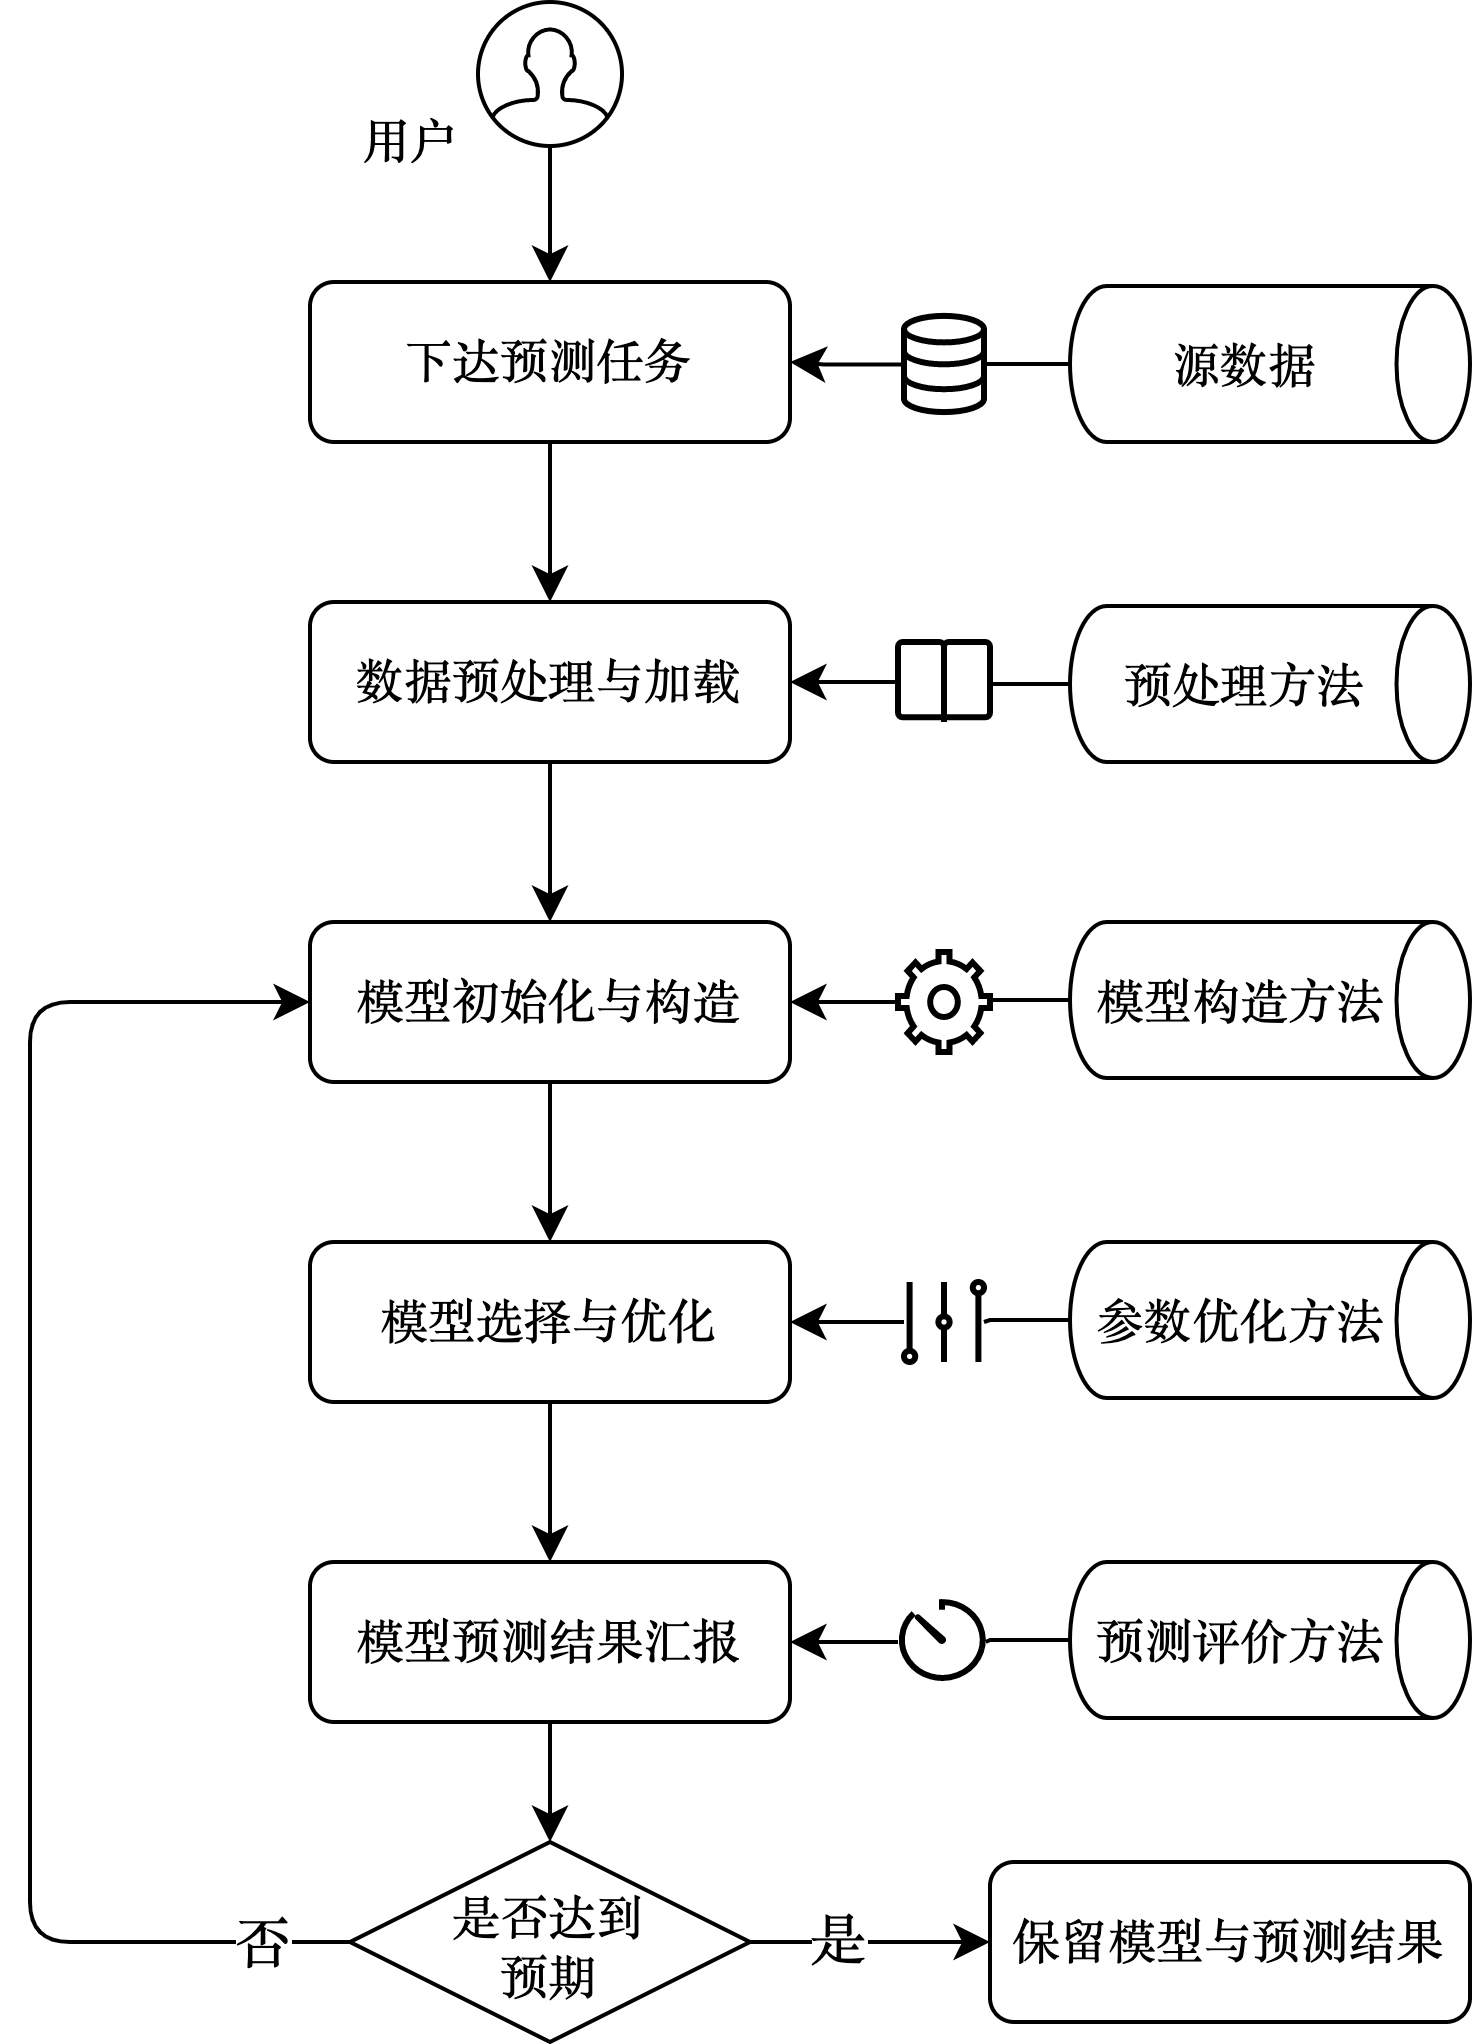
\includegraphics[width=0.8\textwidth]{float/ch.univ/flow.png}
    \caption{框架逻辑流程图\label{fig:ch.univ.flow}}
\end{figure}
\section{框架逻辑流程}
\autoref{fig:ch.univ.flow}展示了本框架的逻辑流程图。该流程图中的步骤说明如下:

(1)用户下达预测任务。基于不同的时间序列预测任务情形,用户收集到所需的时间序列源数据。这些源数据可以是以“txt”、“xlsx”、“csv”和“json”等格式保存的本地文件,也可以是存储在本地或云端数据库系统中的数据库文件。

(2)数据预处理与加载。基于所收集到的源数据,定义继承TaskDataset父类的数据文件Data子类,通过重构“info_config”函数完成时间序列预测任务的基础数据信息设定,利用“sub_config”函数抽取出预测任务所需的时间序列数据,并结合与“info_config”中的信息设定相匹配的预处理方法,完成时间序列数据的异常值处理、归一化、数据集切分等预处理工作,打包预处理数据与对应信息设定并予以加载。

(3)模型初始化与构造。基于使用本框架目标的不同,用户可从内置预测模型方法中选择出合适的模型或自行构造新的模型。针对所选择或设计的模型构造方法,定义继承Model_base父类的模型参数Model子类,通过修改“base_init”函数指定模型构造方法的保存路径与模型类名,通过修改“setting_init”或“setting_modify”函数指定模型参数的初始化设置、模型搜索空间设置和优化器参数设置等参数信息。而后,框架将基于已加载的数据信息和已指定的模型参数信息,自动完成模型的初始化与构造工作。

(4)模型选择与优化。基于已加载的训练集与验证集数据以及已指定的模型参数搜索空间和优化器参数等设置,框架将自动分配计算资源,调用优化器高效进行模型选择过程,完成模型参数的优化。该优化过程不仅包含模型隐藏层神经元数量、激活函数种类和隐藏层层数等模型结构参数,通过本文第5章节所提出的二重特征结构及其编码表示方法,多输入特征选择与优化亦被囊括在内。同时,用户可重构TaskTuner类的“algo_init”函数,灵活选取不同的优化算法,进一步提高模型预测性能。

(5)模型预测结果汇报。基于已加载的测试集数据和已优化的预测模型,框架将基于所设置的重复试验次数与指定的预测准确度指标,自动完成模型测试,并整理模型在当前设置下的预测结果,详细汇报出各预测准确度指标的平均值、标准差、时步误差曲线等信息,同时提供Naive方法的测试结果以做基准参考。若未达预期,则可通过修改模型结构设计、参数搜索空间和优化算法选择等设置,继续调整模型直到符合预期,最终保留模型与预测结果。

\section{小结}
面对复杂多变的时间序列预测需求,为提升时间序列预测建模技术的集成水平与运行效率,本章节在已有优秀模型构造框架与参数优化框架的基础上,设计并开源了一套兼具高集成度与强扩展性的时间序列预测建模框架“OpenForcasting”。
通过对时间序列预测建模框架的用户需求分析,归纳出包含数据管理功能、模型构造功能与模型优化功能在内的核心需求功能,完成了时间序列预测建模框架的系统结构设计与逻辑流程设计。
基于此,本框架内置了不同类别的多种优秀预测模型方法,通过良好的接口设计规范,使得用户能够灵活处理不同结构的时间序列源数据,设计模型结构,调整模型参数和选择优化算法,从而更好解决时间序列预测问题。


